\begin{figure}
  \centering
  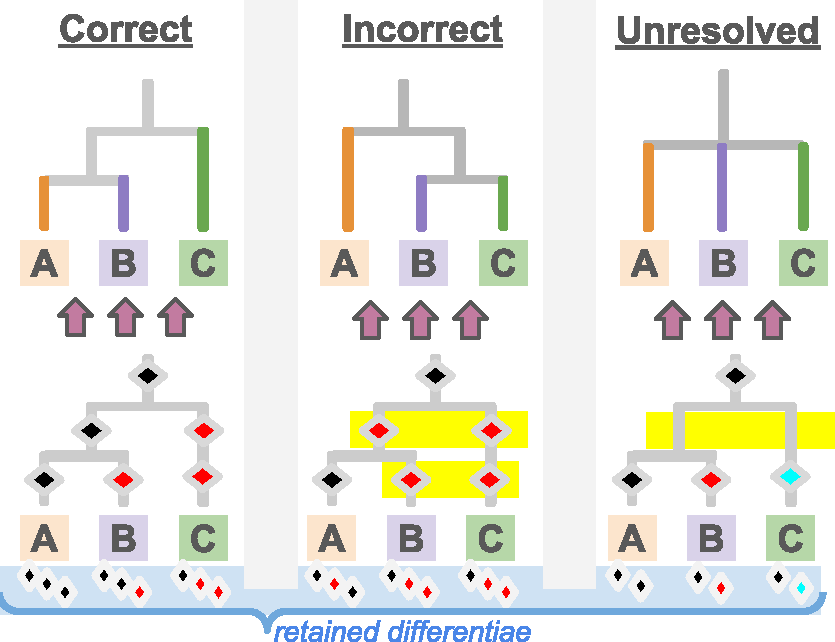
\includegraphics[width=\linewidth]{img/hstrat-failure-modes}
  \caption{%
    \textbf{Differentia structure and reconstruction outcomes.}
    Illustration depicts possible outcomes of reconstruction from hereditary stratigraphy differentia (diamonds) generated and inherited along a two-branch phylogeny (panel bottoms) and resulting reconstruction outcomes (panel tops).
    Diamond placement indicates when differentia were gained and color represents each differentiae's randomly-generated value.
    Diamonds below phylogeny tips summarize inherited hereditary stratigraph record of that taxon.
    \textbf{\textit{Correct reconstruction}} (left panel) occurs when differentia intersperse branching events and differentia value collisions do not occur.
    \textbf{\textit{Incorrect reconstruction}} (center panel) occurs when differentia collisions make unrelated taxa falsely appear related (yellow highlights).
    \textbf{\textit{Unresolved reconstruction}} (i.e., false polytomies; right panel) occurs when differentia do not intersperse branching events but collisions do not occur.
    Note that unresolved reconstructions require differentia size larger than one bit (in order to support $>2$ differentia values), except in the case where more than two differentia records are entirely identical.
  }
  \label{fig:hstrat-failure-modes}
\end{figure}
